\documentclass[border=10pt]{standalone}
\usepackage{pgfplots}
\pgfplotsset{compat=1.18}
\begin{document}
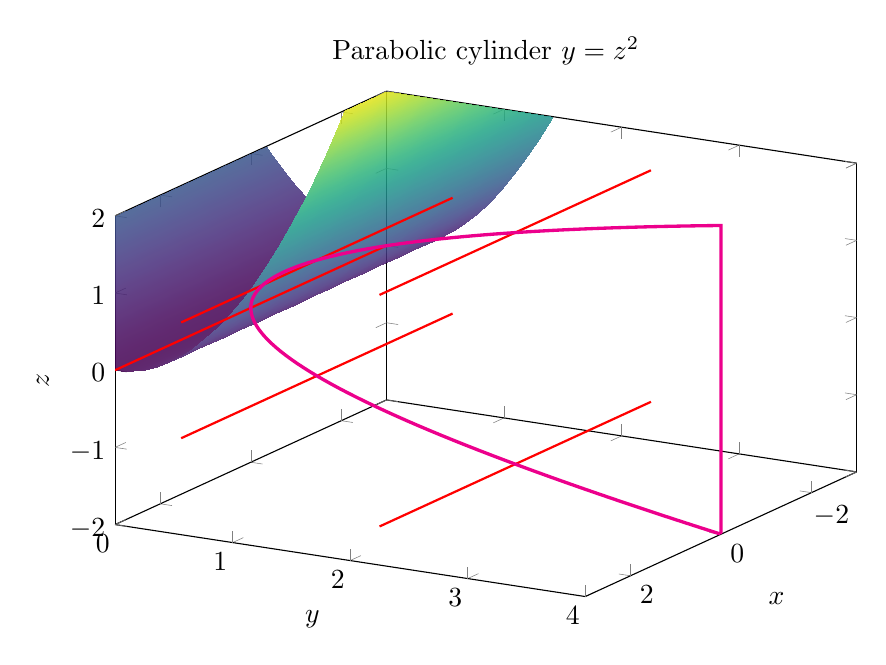
\begin{tikzpicture}
\begin{axis}[
    view={120}{25},
    xlabel=$x$, ylabel=$y$, zlabel=$z$,
    xmin=-3, xmax=3,
    ymin=0, ymax=4,
    zmin=-2, zmax=2,
    title={Parabolic cylinder $y=z^2$},
    width=11cm, height=8cm,
    colormap/viridis,
]
\addplot3[surf, shader=interp, domain=-3:3, domain y=-2:2, samples=40, samples y=40, opacity=0.85] {y^2};
% rulings parallel to x-axis
\addplot3[red, thick, domain=-3:3, samples=2] ({x},{2.25},{-1.5});
\addplot3[red, thick, domain=-3:3, samples=2] ({x},{0.5625},{-0.75});
\addplot3[red, thick, domain=-3:3, samples=2] ({x},{0},{0});
\addplot3[red, thick, domain=-3:3, samples=2] ({x},{0.5625},{0.75});
\addplot3[red, thick, domain=-3:3, samples=2] ({x},{2.25},{1.5});
% generating parabola in the yz-plane
\addplot3[magenta, very thick, domain=-2:2, samples=100] ({0},{x^2},{x});
\end{axis}
\end{tikzpicture}
\end{document}